\begin{figure}[H]
\centering
	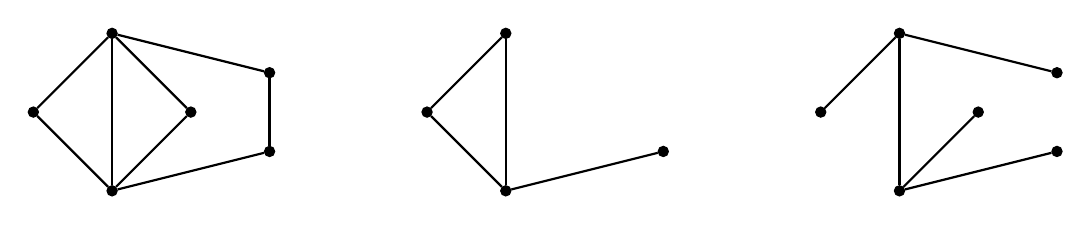
\begin{tikzpicture}

      \tikzset{enclosed/.style={draw, circle, inner sep=0pt, minimum size=.13cm, fill=black}}
% Vertices
	%Hel graf
      	\node[enclosed] (v1) at (0,2) {};
      	\node[enclosed] (v2) at (1,3) {};
    	\node[enclosed] (v3) at (1,1) {};
  	    \node[enclosed] (v4) at (3,1.5) {};
  	    \node[enclosed] (v42) at (3,2.5) {};
  	    \node[enclosed] (v5) at (2,2) {};
  	    
	%Induceret graf
		\node[enclosed] (v6) at (5,2) {};
      	\node[enclosed] (v7) at (6,3) {};
  	    \node[enclosed] (v8) at (6,1) {};
  	    \node[enclosed] (v9) at (8,1.5) {};
  	    
	%Udspændende graf
		\node[enclosed] (v10) at (10,2) {};
      	\node[enclosed] (v11) at (11,3) {};
   	 	\node[enclosed] (v12) at (11,1) {};
  	    \node[enclosed] (v13) at (13,1.5) {};
  	    \node[enclosed] (v132) at (13,2.5) {};
  	    \node[enclosed] (v14) at (12,2) {};
  	    
%Edges
	%Hel graf
		\path[thick] (v1) edge node {} (v2);
		\path[thick] (v1) edge node {} (v3);
		\path[thick] (v3) edge node {} (v4);
		\path[thick] (v3) edge node {} (v5);
		\path[thick] (v4) edge node {} (v42);
		\path[thick] (v2) edge node {} (v42);
		\path[thick] (v2) edge node {} (v5);
		\path[thick] (v2) edge node {} (v3);
		
	%Induceret graf
		\path[thick] (v6) edge node {} (v7);
		\path[thick] (v6) edge node {} (v8);
		\path[thick] (v8) edge node {} (v9);
		\path[thick] (v7) edge node {} (v8);
		
	%Udspændende graf
		\path[thick] (v10) edge node {} (v11);
		\path[thick] (v11) edge node {} (v12);
		\path[thick] (v12) edge node {} (v14);
		\path[thick] (v12) edge node {} (v13);
		\path[thick] (v11) edge node {} (v132);

	\end{tikzpicture}
	\caption{Simpel graf, $G$ (venstre). Induceret delgraf af $G$ (midten). Udspændende delgraf af $G$ (højre).}
	\label{fig:delgraf.eks}
\end{figure}

